\documentclass[12pt]{extreport}
%\usepackage[utf8]{inputenc}
\usepackage{geometry}
    \geometry{
    a4paper,
    total={170mm, 257mm},
    left=20mm,
    top=20mm
    }
    
\usepackage{amsmath}
\usepackage{amssymb}
\usepackage{ulem}
\usepackage{color}
\usepackage{amsthm}
\usepackage{verbatim} 
\usepackage{hyperref}
\usepackage{enumitem}
\usepackage{siunitx}
\usepackage{graphicx}
\usepackage[parfill]{parskip}


\newenvironment{solution}
  {\renewcommand\qedsymbol{$\blacksquare$}\begin{proof}[Solution]}
  {\end{proof}}

% Defining commands:
\newcommand{\R}{\mathbb{R}}
\newcommand{\exhat}{\hat{e}_x}
\newcommand{\eyhat}{\hat{e}_y}
\newcommand{\ezhat}{\hat{e}_z}
\newcommand{\harmexp}{e^{-\frac{m\omega x^2}{2 \hbar}}}
\newcommand*{\I}{\imath}
\newcommand*{\J}{\jmath}


\title{Physics II Class Notes}
\author{Professor: Kunal Ghosh, Compiled: Skanda Kaashyap}
\date{Summer I, 2019}

\begin{document}

\maketitle
\chapter{Electric Field}
\section{What is the electric field?}
On 5/21/19, we discussed the electric field. The electric field is a bit more abstract than some of the other concepts that we've dealt with so far; that is to say, it's not something that you can directly feel, like an electric force. It's often useful to think about the electric field the same way we often thinka about the gravitational field: like a trampoline. Imagine negative charges pushing down on the surface of the trampoline and positive charges pulling up. This is a helpful visual.  \\

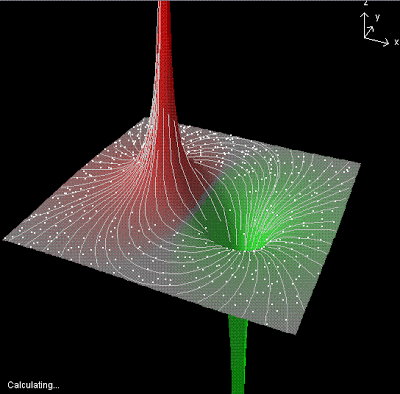
\includegraphics[]{efield.PNG}

\section{How to Compute the Electric Field}
 The electric field is given by $$\vec E = \frac{kQ}{|r|^2}\hat r,$$ where $\hat r$ points from the charge inducing the field to the location at which you would like to measure the field. You will no doubt notice its striking resemblance to the Coulomb force, which is given by 
	\begin{align}
		\vec F_{12} = \frac{k Q q}{|r_{21}|^2} \hat r_{21}
	\end{align}
In fact, the $E$ field is really $\vec{E} = \vec F/q,$ which can be interpreted as ``force per unit charge.'' One way to think about it is that in the same way that volume density is mass per unit volume, this is, in some sense, a ``force density.'' It describes how the space around the object itself changes; it describes a \textit{field.}

\section{Finding $\vec E$ field Around Different Objects}
In class, we discussed obtaining the electric field around various different objects. Try to see if you can find the electric field expression for the following objects with constant linear charge density.
	\begin{itemize}
		\item Straight line
		\item Ring
		\item Disk
		\item Sphere
	\end{itemize}
Try to also see if you can obtain the near and far field limits for each of these objects. 

\subsection{Solving Technique}
Here we will outline how to go about solving the E field for a straight line of charge with constant linear charge density. The problem solving method does not change for other geometries, only the mechanics. That being said, it's still useful to try those, since you might be expected to know how to compute different types of integrals, including ones with trig substitutions. 

\begin{solution}

	\textbf{What do we know?}

	So far, we know that the E field expression for a point charge is given by $\vec E = (kq/r^2) \hat r.$ 

	\textbf{But we don't have a point charge!}
	But since we don't have a point charge here, we can break up the line into an infinite number of point charges. We can compute the E field $d\vec E$ for a single charge differential $dQ$ and sum them up to get our field for the line.

	The integral becomes 
	\begin{align*}
		d\vec E &= \frac{k dQ}{|r|^2} \hat r \\
		\Rightarrow \vec E &= \int \frac{k dQ}{|r|^2} \hat r
	\end{align*}
	Often times, $dQ$ can be expressed as a density multiplied by a length differential, like $dQ = \lambda dx$ in this case.
\end{solution}

\section{Natural E-Field Calculations}
In this section, I want to briefly discuss how calculating the $\vec E$ field expression for a uniform charge is a natural starting point to ultimately perform an integral to obtain the $\vec E$ field for a full, 3D object, assuming that we don't want to use Gauss's Law.

We calculated the $\vec E$ field for a line of charge by performing the following integral: $$\vec E = \int \frac{\lambda k}{|r|^2} \hat r dx.$$ Now, if we imagine a singular ``rod'' and turning contorting it into a circle, then we have a ring. The geometry changes, but you are still, at the of the day, taking a line integral, so it will look of the form above. Add a bunch of rings of varying sizes and you get a disk; add a bunch of disks of the same size, you get a cylinder. Add a bunch of disks of \textit{varying} sizes, you get a sphere. 

My point here is that even though the geometries of the objects are changing, the mechanics of performing an integral stays the same and the fundamental property that performing an integral allows you to perceive higher dimensions also holds. This means that a ring of charge is just a line of charge, and adding a bunch of points (0 dimensions) gets you a 1 dimensional object (a line), adding a bunch of lines (1 dimension) gets you a plane, adding a bunch of rings gets you a disk, etc.


% \chapter{Dipoles}
% Dipoles are a very interesting and exciting application of some of the most fundamental concepts in E\&M, the very same concepts that we've been learning so far. So far, we've learned of the 

% \chapter{Exploring the Similarities Between Gravitational and Electrostatic Forces}
% The gravitational force is given by $$F_g = -\frac{GMm}{R^2} \hat r.$$ The electrostatic force is given by $$F_e = -\frac{k Q q}{r^2} \hat r.$$

\chapter{Gauss's Law}
\section{Definition}
Gauss's Law is defined by
	\begin{align}
		\oint_A \vec E \cdot d \vec A = \frac{q_{enc}}{\epsilon_0}
	\end{align}
	
\section{Meaning}
All Gauss's Law is saying is the following: ``If we take the portion of the $\vec E$ field that is normal to the surface and we sum it up across the area of the surface, it will be proportional to the charge enclosed.'' Let's construct a surface to trap the $\vec E$ field vectors for the charge that \textit{we're interested in} and sum them up. The number of $\vec E$ field vectors we trap should be proportional to the magnitude of the thing causing those vectors in the first place.

\section{Application}
This is a really simple and elegant statement because it reduces a lot of complexity in the system. Using Gauss's law, we only have to worry about 3 things: 
	\begin{enumerate}
		\item Charge enclosed
		\item Gaussian surface
		\item Magnitude of charge, direction of $\vec E$ field vectors.
	\end{enumerate}
Once we have these 3 things, it's just the matter of computing a surface integral. I think a great example and practice problem for this was the special problem in homework 3. It forced you to think hard about what your Gaussian surface would look like. You had to draw the Gaussian surface not at the exact location of the shell, but a little bit above so you could encapsulate the information that the inner part of the shell was telling you. Otherwise, you would be given information about what was going on in the rod. Remember, Gauss's law only tells you about the \textit{charge enclosed} within the Gaussian surface.

\chapter{Class Notes}

\section{Notes 5/22/19}
QABS = Question Asked By Student
\begin{itemize}
	\item Recall, the force of particle 2 on 1 is given by $F_{1,2}$.
	\item Question: what are the units of the electric field? Answer: Well, what would happen if you had multiple charges?
	\item How do we solve the uniformly charged rod?
	\item QABS: How do we visualize the tiny charge differentials?
	\item QABS: What is $dr?$
	\item QABS: How do we find charge density? Ans: $$dQ = \frac{dy}{L} Q_0,$$ where $Q_0$ is the total charge.

	\begin{solution}
		The rule is always the same. We want to find the sum $$\vec F = \sum_{i} \vec E_i q_i.$$

		Recall, the electric field is a \textit{vector}. 

		That being said, let's either guess or predict the direction of the electric field/force.

		So we can split things up into the positive and negative directions.

		We found the E field differential. After we find the E field differential, we want to integrate over the whole thing. We want to find the total E field. 

		Important things to keep an eye out basically all the time:
		\begin{itemize}
			\item Look at limits.
			\item Look for symmetries.
			\item You can always pull out constants.
		\end{itemize}

		Basically, when we have these squared looking integrals, we want to see if we can rewrite these in terms of trigonometric identities. 

		Ask yourself: What trig substitutions have you seen in class?

		Things to check after solving a problem:
		\begin{enumerate}
			\item Does it make sense? Are the vectors pointing in the right directions? Do we have scalars when we should have vectors? Is it in roughly the same order of magnitude?
			\item Are the dimensions correct?	
			\item Check close field and far field limits.
		\end{enumerate}			

	\end{solution}
\end{itemize}

% \section{Notes 5/23/19}
% These notes are taken on paper and sho`uld be transferred to the manuscript.

\section{Notes 5/24/19}
\begin{itemize}
	\item Solve the electric field for a hollowed out disk. Solution: just find the E field for big disk, small disk, then subtract. Again, this uses the \textit{superposition principle.}

	% \item Our final solution for this problem should yield $$\vec E_p = \frac{1}{4 \pi} \frac{2 Q_0}{R^2}$$
	\item QABS: 

	\item It is very important to recall the \textbf{Taylor expansion relation} $(1 + \alpha)^\beta = 1+ \alpha \beta$ as long as $\alpha << 1.$

	\item In order to find close and far field limits, if we have denominators like $(a + b)^n,$ we can always reduce to obtain an expression of the form $(1 + \alpha)^\beta.$

	% \item Q: how does the binomial theorem lead to the Taylor expansion of $(1+\alpha)^\beta?$

	\item Question to consider: In order to show that the $\vec E$ field inside a spherical shell is zero, can we imagine a ring, rotate it around its axis, and then integrate? 

	\item Summary of what we did today:
		\begin{itemize}
			\item We solved the disk with hole.
			\item We solved the near and far field limits of the disk. In so doing, we introduced the binomial theorem/Taylor expansion of $(1+\alpha)^\beta.$ How can we prove/derive $(1+\alpha)^\beta$ with the binomial theorem?
			\item We discussed the electric field inside a hollow sphere and a outside a hollow sphere. 
			\item Discussed the motion and electric field inside a uniformly charged, nonconducting sphere. This is basically the motion inside of the earth. 

			\item What if we had an electric force that varied as $\frac 1 {r^3}?$ More generally, what if it varied as $1/r^n?$

			\item Introduced Gauss's Law.

			\item If we construct a ``Gaussian surface.'' If we perform the following calculation, $$\oint \vec E \cdot d \vec A = \frac{q_{enc}}{\epsilon_0}.$$

			% \item (needs an intuitive explanation: naie) why does the e field point radially outwards from a point charge?
			% \textit{answer: a straight line is the }
		\end{itemize}
\end{itemize}

\section{Notes 5/28/19}
	\begin{itemize}
		\item Starting/looking at Gauss's law: $\oint \vec E \cdot d\vec A = q_{enc}/\epsilon_0.$

		\item What would the electric field be around a rod that is not infinitely long? 

		\item We also introduced the cylindrical coordinate system. The spherical coordinate system is characterized by $\rho, \phi, z.$ 

		\item The conversion rate is given by 
			\begin{align*}
				x &= \rho \cos \phi \\
				y &= \rho \sin \phi \\
				z &= z
			\end{align*}

		\item The basis vectors are given by: 
			\begin{align*}
				\hat \rho &= \cos \phi \hat \imath  + \sin \phi \hat \jmath \\
				\hat \phi &= -\sin \phi \hat \imath + \cos \phi \hat \jmath \\
				\hat z &= \hat z
			\end{align*}

		\item The generalized expression for the electric field in cylindrical coordinates is going to be: $$\hat E_p = \hat \rho E_\rho(\rho, \phi, z) + \hat \phi E_\phi(\rho, \phi, z) + \hat z E_z (\rho, \phi, z).$$

		\item Use Coulomb's law, basis of electric attraction and repulision to reduce $\hat A, \hat B, \hat C$ as much as possible.

		\item Consider an infinitely long, positively charged rod. In such a situation, a point charge some distance $\rho$ away will feel a force necessarily in the $\hat \rho$ direction.	

		\item The rod looks the same anywhere in $\hat \phi$ direction and the $\hat z$ direction.

		\item Problem solving algorithm:
			\begin{enumerate}
				\item Look for symmetries. This is useful in not just E\&M, but basically everywhere.

				\item Find a coordinate system that also has the same symmetries. For example, with a rod, a cylindrical Gaussian surface is suitable.

				\item Remember, the generalized $\vec E$ field is given by 
				\begin{align*}
					\vec E_p &= \hat A E_A(A, B, C) \\
							 &+ \hat B E_B(A, B, C) \\
							 &+ \hat C E_C(A, B, C)
				\end{align*}

				\item Use Coulomb's law to figure out electric attractions and repulsions. This will allow you to determine which components of the $\vec E$ field should remain.

				\item Use symmetry arguments to reduce the number of variables.

				\item Then simply solve for $|\vec E|.$

				\item Basically, when choosing our Gaussian surface, we want to find something whose $\vec E \cdot d \vec A$ has no angular component.

				\item Find \textit{representative points.} These are points that ``represent'' each unique surface. If our surface is a cylinder, there are 3 main representative points: the body of the cylinder, and the two bases. Since this is not continuous, you will need 3 integrals.

				\item Solve all these integrals.
			\end{enumerate} 
	\end{itemize}

\section{Notes 5/29/19}
	\begin{itemize}
		\item So what are some of the benefits of Gauss's Law?
		Well consider finding the E field of a solid charged sphere. If you had to use the tools you learned in chapter 21, this would be a much more difficult calculus problem. You will have to decompose the sphere into a series of disks and integrate the E field through the entire sphere since you already know the E field for a disk. But now, we can instead use Gauss's Law.

		\item We introduce spherical coordinates: The E field in spherical coordinates is described by:
		\begin{align*}
			\vec E_p &= \hat r E_r(r, \theta, \phi) \\
				     &+ \hat \theta E_\theta(r, \theta, \phi) \\
				     &+ \hat \phi E_\phi(r, \theta, \phi)
		\end{align*}

		\item The conversion rate for spherical coordinates is given by:
		\begin{align*}
			x &= r \cos \phi \sin \theta \hat x \\
			y &= r \sin \phi \sin \theta \hat y \\
			z &= r \cos \theta \hat z
		\end{align*}

		Therefore, the spherical basis vectors are given by: 
		\begin{align*}
			\hat r &= \cos \phi \sin \theta \hat x + \sin \phi \sin \theta \hat y + \cos \theta \hat z \\
			\hat \phi &= \frac{d \hat r/d\phi}{|d \hat r/d\phi|} = \sin \phi \hat x + \cos \phi \hat y + 0 \hat z \\
			\hat \theta &= \frac{d \hat r/d\theta}{|d \hat r/d\theta|} = \cos \phi \cos \theta \hat x + \sin \phi \cos \theta \hat y - \sin \theta \hat z
		\end{align*}

		\item Problem solving steps:
		\begin{enumerate}
			\item Expect $\vec E$ to go in the $\hat r$ direction.
			\item We're probably going to be using spherical polar coordinates.
			\item Think about what would happen empirically/experimentally.
			\item Make as many symmetry arguments as possible to reduce your calculations.
			\item Choose a fish net such that the fish net contains all the ``fish.'' What this means is that we want to choose a Gaussian surface such that the surface encloses all the points.
			\item Choose your ``representative points.''
			\item Always remember, laziness is crucial to solving Gauss's law problems. Without it, you will most definitely fail.
			\item In all seriousness, try to make your own life as easy as possible. Reduce as much as possible, pick the most convenient Gaussian surface as possible, and ensure that your chosen Gaussian surface encapsulates all the information you want. That is, you are interested in what is going on WITHIN the Gaussian sphere, but are not interested in ANY less or ANY more.
		\end{enumerate}

		\item We are saying that the E field must only be in the $z$ direction and that the E field relies only on $\vec E_p = \hat z E(z).$

		\item Ask yourself: What are the 4 requirements of determining a Gaussian surface?
	\end{itemize}


\chapter{Fun Problems}
\section{Dipoles and Charged Rods: From Lectures 5/20 - 5/22}
	\begin{enumerate}
		\item
		Consider a uniformly charged rod of linear density: $$\rho = nx,$$ or parabolic density: $$\rho = nx^2,$$ general case for polynomial density, where $$\rho = nx^p.$$ Find the electric field a distance $d$ from the center of the rod. 

		\item
		What if we made a dipole out of two rods? What would the electric field around that look like?

		\item
		What is the electric field of a dipole with two rods of varying charge density?

		\item
		Consider a rod, where half of it is positive and the other half is negative. At which point is it justifiable to say that the rod becomes a dipole? Is it justifiable at all? This question is motivated by the fact that a rod at a far field limit begins looking like a point.

		\item
		Consider an infinitely long and wide charged plane. The density is given by $\gamma,$ given in units of $\mu$C$/$m$^2.$ What is the electric field due to \textit{only a single side of the sheet?}

	\end{enumerate}

% \chapter{Grading Observations}
% \section{Common Mistakes and Things We Should Emphasize Based on Quiz 1}
% 	\begin{itemize}
% 		\item People forgot units...A LOT. Emphasize that we care about units because units are fundamental to understanding whether or not our quantity makes physical sense and is crucial to being able to check our problems afterwards. If we do not check our units, we are performing meaningless calculations and are no longer doing physics.

% 		\item The correct form of Coulomb's Law is $$\vec F_{12} = \frac{k q_1 q_2}{|r_{12}|^2} \hat r_{21}.$$ People were confused with whether or not there should be an absolute value sign around $|q_1 q_2|.$ It should be emphasized that the direction of the force is fundamentally obtained from 2 things: the location in space of each of the objects and the charge of both objects. If we agree that we are always going to draw the vector from the object that causes the force to the object that feels the force, (in this case object 2 causes the force and our vector $\hat r_{21}$ goes from item 2 to item 1), then we only need to worry about the sign. If we get our signs right, then we can be sure that our force expression is correct. This can be verified by showing the direction of the force for 2 positive test charges. The force that object 2 feels due to object 1 will be a positive quantity with a vector $\hat r_{21}.$

% 		\item Vector quantities should be expressed as vectors. People should ensure that their vectors are pointing in the correct direction. 
% 	\end{itemize}

\end{document}